% Options for packages loaded elsewhere
\PassOptionsToPackage{unicode}{hyperref}
\PassOptionsToPackage{hyphens}{url}
\PassOptionsToPackage{dvipsnames,svgnames,x11names}{xcolor}
%
\documentclass[
  letterpaper,
  DIV=11,
  numbers=noendperiod]{scrartcl}

\usepackage{amsmath,amssymb}
\usepackage{iftex}
\ifPDFTeX
  \usepackage[T1]{fontenc}
  \usepackage[utf8]{inputenc}
  \usepackage{textcomp} % provide euro and other symbols
\else % if luatex or xetex
  \usepackage{unicode-math}
  \defaultfontfeatures{Scale=MatchLowercase}
  \defaultfontfeatures[\rmfamily]{Ligatures=TeX,Scale=1}
\fi
\usepackage{lmodern}
\ifPDFTeX\else  
    % xetex/luatex font selection
\fi
% Use upquote if available, for straight quotes in verbatim environments
\IfFileExists{upquote.sty}{\usepackage{upquote}}{}
\IfFileExists{microtype.sty}{% use microtype if available
  \usepackage[]{microtype}
  \UseMicrotypeSet[protrusion]{basicmath} % disable protrusion for tt fonts
}{}
\makeatletter
\@ifundefined{KOMAClassName}{% if non-KOMA class
  \IfFileExists{parskip.sty}{%
    \usepackage{parskip}
  }{% else
    \setlength{\parindent}{0pt}
    \setlength{\parskip}{6pt plus 2pt minus 1pt}}
}{% if KOMA class
  \KOMAoptions{parskip=half}}
\makeatother
\usepackage{xcolor}
\setlength{\emergencystretch}{3em} % prevent overfull lines
\setcounter{secnumdepth}{-\maxdimen} % remove section numbering
% Make \paragraph and \subparagraph free-standing
\makeatletter
\ifx\paragraph\undefined\else
  \let\oldparagraph\paragraph
  \renewcommand{\paragraph}{
    \@ifstar
      \xxxParagraphStar
      \xxxParagraphNoStar
  }
  \newcommand{\xxxParagraphStar}[1]{\oldparagraph*{#1}\mbox{}}
  \newcommand{\xxxParagraphNoStar}[1]{\oldparagraph{#1}\mbox{}}
\fi
\ifx\subparagraph\undefined\else
  \let\oldsubparagraph\subparagraph
  \renewcommand{\subparagraph}{
    \@ifstar
      \xxxSubParagraphStar
      \xxxSubParagraphNoStar
  }
  \newcommand{\xxxSubParagraphStar}[1]{\oldsubparagraph*{#1}\mbox{}}
  \newcommand{\xxxSubParagraphNoStar}[1]{\oldsubparagraph{#1}\mbox{}}
\fi
\makeatother

\usepackage{color}
\usepackage{fancyvrb}
\newcommand{\VerbBar}{|}
\newcommand{\VERB}{\Verb[commandchars=\\\{\}]}
\DefineVerbatimEnvironment{Highlighting}{Verbatim}{commandchars=\\\{\}}
% Add ',fontsize=\small' for more characters per line
\usepackage{framed}
\definecolor{shadecolor}{RGB}{241,243,245}
\newenvironment{Shaded}{\begin{snugshade}}{\end{snugshade}}
\newcommand{\AlertTok}[1]{\textcolor[rgb]{0.68,0.00,0.00}{#1}}
\newcommand{\AnnotationTok}[1]{\textcolor[rgb]{0.37,0.37,0.37}{#1}}
\newcommand{\AttributeTok}[1]{\textcolor[rgb]{0.40,0.45,0.13}{#1}}
\newcommand{\BaseNTok}[1]{\textcolor[rgb]{0.68,0.00,0.00}{#1}}
\newcommand{\BuiltInTok}[1]{\textcolor[rgb]{0.00,0.23,0.31}{#1}}
\newcommand{\CharTok}[1]{\textcolor[rgb]{0.13,0.47,0.30}{#1}}
\newcommand{\CommentTok}[1]{\textcolor[rgb]{0.37,0.37,0.37}{#1}}
\newcommand{\CommentVarTok}[1]{\textcolor[rgb]{0.37,0.37,0.37}{\textit{#1}}}
\newcommand{\ConstantTok}[1]{\textcolor[rgb]{0.56,0.35,0.01}{#1}}
\newcommand{\ControlFlowTok}[1]{\textcolor[rgb]{0.00,0.23,0.31}{\textbf{#1}}}
\newcommand{\DataTypeTok}[1]{\textcolor[rgb]{0.68,0.00,0.00}{#1}}
\newcommand{\DecValTok}[1]{\textcolor[rgb]{0.68,0.00,0.00}{#1}}
\newcommand{\DocumentationTok}[1]{\textcolor[rgb]{0.37,0.37,0.37}{\textit{#1}}}
\newcommand{\ErrorTok}[1]{\textcolor[rgb]{0.68,0.00,0.00}{#1}}
\newcommand{\ExtensionTok}[1]{\textcolor[rgb]{0.00,0.23,0.31}{#1}}
\newcommand{\FloatTok}[1]{\textcolor[rgb]{0.68,0.00,0.00}{#1}}
\newcommand{\FunctionTok}[1]{\textcolor[rgb]{0.28,0.35,0.67}{#1}}
\newcommand{\ImportTok}[1]{\textcolor[rgb]{0.00,0.46,0.62}{#1}}
\newcommand{\InformationTok}[1]{\textcolor[rgb]{0.37,0.37,0.37}{#1}}
\newcommand{\KeywordTok}[1]{\textcolor[rgb]{0.00,0.23,0.31}{\textbf{#1}}}
\newcommand{\NormalTok}[1]{\textcolor[rgb]{0.00,0.23,0.31}{#1}}
\newcommand{\OperatorTok}[1]{\textcolor[rgb]{0.37,0.37,0.37}{#1}}
\newcommand{\OtherTok}[1]{\textcolor[rgb]{0.00,0.23,0.31}{#1}}
\newcommand{\PreprocessorTok}[1]{\textcolor[rgb]{0.68,0.00,0.00}{#1}}
\newcommand{\RegionMarkerTok}[1]{\textcolor[rgb]{0.00,0.23,0.31}{#1}}
\newcommand{\SpecialCharTok}[1]{\textcolor[rgb]{0.37,0.37,0.37}{#1}}
\newcommand{\SpecialStringTok}[1]{\textcolor[rgb]{0.13,0.47,0.30}{#1}}
\newcommand{\StringTok}[1]{\textcolor[rgb]{0.13,0.47,0.30}{#1}}
\newcommand{\VariableTok}[1]{\textcolor[rgb]{0.07,0.07,0.07}{#1}}
\newcommand{\VerbatimStringTok}[1]{\textcolor[rgb]{0.13,0.47,0.30}{#1}}
\newcommand{\WarningTok}[1]{\textcolor[rgb]{0.37,0.37,0.37}{\textit{#1}}}

\providecommand{\tightlist}{%
  \setlength{\itemsep}{0pt}\setlength{\parskip}{0pt}}\usepackage{longtable,booktabs,array}
\usepackage{calc} % for calculating minipage widths
% Correct order of tables after \paragraph or \subparagraph
\usepackage{etoolbox}
\makeatletter
\patchcmd\longtable{\par}{\if@noskipsec\mbox{}\fi\par}{}{}
\makeatother
% Allow footnotes in longtable head/foot
\IfFileExists{footnotehyper.sty}{\usepackage{footnotehyper}}{\usepackage{footnote}}
\makesavenoteenv{longtable}
\usepackage{graphicx}
\makeatletter
\newsavebox\pandoc@box
\newcommand*\pandocbounded[1]{% scales image to fit in text height/width
  \sbox\pandoc@box{#1}%
  \Gscale@div\@tempa{\textheight}{\dimexpr\ht\pandoc@box+\dp\pandoc@box\relax}%
  \Gscale@div\@tempb{\linewidth}{\wd\pandoc@box}%
  \ifdim\@tempb\p@<\@tempa\p@\let\@tempa\@tempb\fi% select the smaller of both
  \ifdim\@tempa\p@<\p@\scalebox{\@tempa}{\usebox\pandoc@box}%
  \else\usebox{\pandoc@box}%
  \fi%
}
% Set default figure placement to htbp
\def\fps@figure{htbp}
\makeatother

\KOMAoption{captions}{tableheading}
\makeatletter
\@ifpackageloaded{caption}{}{\usepackage{caption}}
\AtBeginDocument{%
\ifdefined\contentsname
  \renewcommand*\contentsname{Table of contents}
\else
  \newcommand\contentsname{Table of contents}
\fi
\ifdefined\listfigurename
  \renewcommand*\listfigurename{List of Figures}
\else
  \newcommand\listfigurename{List of Figures}
\fi
\ifdefined\listtablename
  \renewcommand*\listtablename{List of Tables}
\else
  \newcommand\listtablename{List of Tables}
\fi
\ifdefined\figurename
  \renewcommand*\figurename{Figure}
\else
  \newcommand\figurename{Figure}
\fi
\ifdefined\tablename
  \renewcommand*\tablename{Table}
\else
  \newcommand\tablename{Table}
\fi
}
\@ifpackageloaded{float}{}{\usepackage{float}}
\floatstyle{ruled}
\@ifundefined{c@chapter}{\newfloat{codelisting}{h}{lop}}{\newfloat{codelisting}{h}{lop}[chapter]}
\floatname{codelisting}{Listing}
\newcommand*\listoflistings{\listof{codelisting}{List of Listings}}
\makeatother
\makeatletter
\makeatother
\makeatletter
\@ifpackageloaded{caption}{}{\usepackage{caption}}
\@ifpackageloaded{subcaption}{}{\usepackage{subcaption}}
\makeatother

\usepackage{bookmark}

\IfFileExists{xurl.sty}{\usepackage{xurl}}{} % add URL line breaks if available
\urlstyle{same} % disable monospaced font for URLs
\hypersetup{
  pdftitle={World Development Indicators},
  pdfauthor={Nick Richards},
  colorlinks=true,
  linkcolor={blue},
  filecolor={Maroon},
  citecolor={Blue},
  urlcolor={Blue},
  pdfcreator={LaTeX via pandoc}}


\title{World Development Indicators}
\author{Nick Richards}
\date{2025-02-26}

\begin{document}
\maketitle


\begin{Shaded}
\begin{Highlighting}[]
\ImportTok{import}\NormalTok{ pandas }\ImportTok{as}\NormalTok{ pd}

\NormalTok{file\_path }\OperatorTok{=} \StringTok{"/Users/nicholasrichards/Desktop/QTM\_350/wdi.csv"}
\NormalTok{df\_wdi }\OperatorTok{=}\NormalTok{ pd.read\_csv(file\_path)}
\NormalTok{df\_wdi.head}
\end{Highlighting}
\end{Shaded}

\begin{verbatim}
<bound method NDFrame.head of                    country  inflation_rate  exports_gdp_share  \
0              Afghanistan             NaN          18.380042   
1                  Albania        6.725203          37.197085   
2                  Algeria        9.265516          30.808979   
3           American Samoa             NaN          46.957520   
4                  Andorra             NaN                NaN   
..                     ...             ...                ...   
212  Virgin Islands (U.S.)             NaN          97.367295   
213     West Bank and Gaza        3.741224          18.436253   
214            Yemen, Rep.             NaN                NaN   
215                 Zambia       10.993204          40.193998   
216               Zimbabwe      104.705171          27.872171   

     gdp_growth_rate  gdp_per_capita  adult_literacy_rate  \
0          -6.240172      357.261153                  NaN   
1           4.826688     6846.426143            98.500000   
2           3.600000     4961.552577                  NaN   
3           1.735016    18017.458938                  NaN   
4           9.564612    42414.059009                  NaN   
..               ...             ...                  ...   
212        -1.311232    44320.909186                  NaN   
213         4.082760     3799.955270            98.000000   
214              NaN      615.702079                  NaN   
215         5.211224     1447.123101                  NaN   
216         6.139263     2040.552459            89.849998   

     primary_school_enrolment_rate  education_expenditure_gdp_share  \
0                              NaN                              NaN   
1                        96.371231                         2.744330   
2                       108.343933                         4.749247   
3                              NaN                              NaN   
4                        90.147346                         2.647290   
..                             ...                              ...   
212                            NaN                              NaN   
213                      91.764587                              NaN   
214                            NaN                              NaN   
215                            NaN                         3.582595   
216                      95.789907                              NaN   

     measles_immunisation_rate  health_expenditure_gdp_share  \
0                         56.0                           NaN   
1                         86.0                           NaN   
2                         79.0                           NaN   
3                          NaN                           NaN   
4                         98.0                           NaN   
..                         ...                           ...   
212                        NaN                           NaN   
213                       97.0                           NaN   
214                       53.0                           NaN   
215                       90.0                           NaN   
216                       90.0                           NaN   

     income_inequality  unemployment_rate  life_expectancy  total_population  
0                  NaN             14.100        62.879000        40578842.0  
1                  NaN             10.137        76.833000         2777689.0  
2                  NaN             12.346        77.129000        45477389.0  
3                  NaN                NaN              NaN           48342.0  
4                  NaN                NaN              NaN           79705.0  
..                 ...                ...              ...               ...  
212                NaN             13.007        80.319512          105413.0  
213                NaN             24.420        73.444000         5043612.0  
214                NaN             17.363        63.720000        38222876.0  
215               51.5              5.995        61.803000        20152938.0  
216                NaN             10.087        59.391000        16069056.0  

[217 rows x 14 columns]>
\end{verbatim}

\begin{Shaded}
\begin{Highlighting}[]
\BuiltInTok{print}\NormalTok{(df\_wdi[}\StringTok{\textquotesingle{}inflation\_rate\textquotesingle{}}\NormalTok{].describe())}
\BuiltInTok{print}\NormalTok{(df\_wdi[}\StringTok{\textquotesingle{}gdp\_per\_capita\textquotesingle{}}\NormalTok{].describe())}
\BuiltInTok{print}\NormalTok{(df\_wdi[}\StringTok{\textquotesingle{}unemployment\_rate\textquotesingle{}}\NormalTok{].describe())}
\end{Highlighting}
\end{Shaded}

\begin{verbatim}
count    173.000000
mean      12.404067
std       19.467053
min       -6.687321
25%        5.518129
50%        7.930929
75%       11.665567
max      171.205491
Name: inflation_rate, dtype: float64
count       207.000000
mean      20520.336828
std       30640.741594
min         250.634225
25%        2599.752468
50%        7606.237525
75%       27542.145523
max      226052.001905
Name: gdp_per_capita, dtype: float64
count    186.000000
mean       7.227344
std        5.844462
min        0.130000
25%        3.478000
50%        5.334000
75%        9.261750
max       35.359000
Name: unemployment_rate, dtype: float64
\end{verbatim}

\subsection{Exploratory Data Analysis}\label{exploratory-data-analysis}

The dataset contains GDP, Population, and Unemployment Rate statistics.
Below are key statistics: - \textbf{Inflation Rate}: count 173.000000
mean 12.404067 std 19.467053 min -6.687321 25\% 5.518129 50\% 7.930929
75\% 11.665567 max 171.205491 dtype: float64 - \textbf{GDP Per Capita}:
count 207.000000 mean 20520.336828 std 30640.741594 min 250.634225 25\%
2599.752468 50\% 7606.237525 75\% 27542.145523 max 226052.001905 dtype:
float64 - \textbf{Unemployment Rate}: count 186.000000 mean 7.227344 std
5.844462 min 0.130000 25\% 3.478000 50\% 5.334000 75\% 9.261750 max
35.359000 dtype: float64

\begin{Shaded}
\begin{Highlighting}[]
\ImportTok{import}\NormalTok{ matplotlib.pyplot }\ImportTok{as}\NormalTok{ plt}

\NormalTok{plt.figure(figsize}\OperatorTok{=}\NormalTok{(}\DecValTok{8}\NormalTok{,}\DecValTok{5}\NormalTok{))}
\NormalTok{plt.scatter(df\_wdi[}\StringTok{\textquotesingle{}gdp\_per\_capita\textquotesingle{}}\NormalTok{], df\_wdi[}\StringTok{\textquotesingle{}unemployment\_rate\textquotesingle{}}\NormalTok{])}
\NormalTok{plt.title(}\StringTok{"GDP vs. Unemployment Rate"}\NormalTok{)}
\NormalTok{plt.xlabel(}\StringTok{"GDP"}\NormalTok{)}
\NormalTok{plt.ylabel(}\StringTok{"Unemployment Rate"}\NormalTok{)}
\NormalTok{plt.show()}
\end{Highlighting}
\end{Shaded}

\pandocbounded{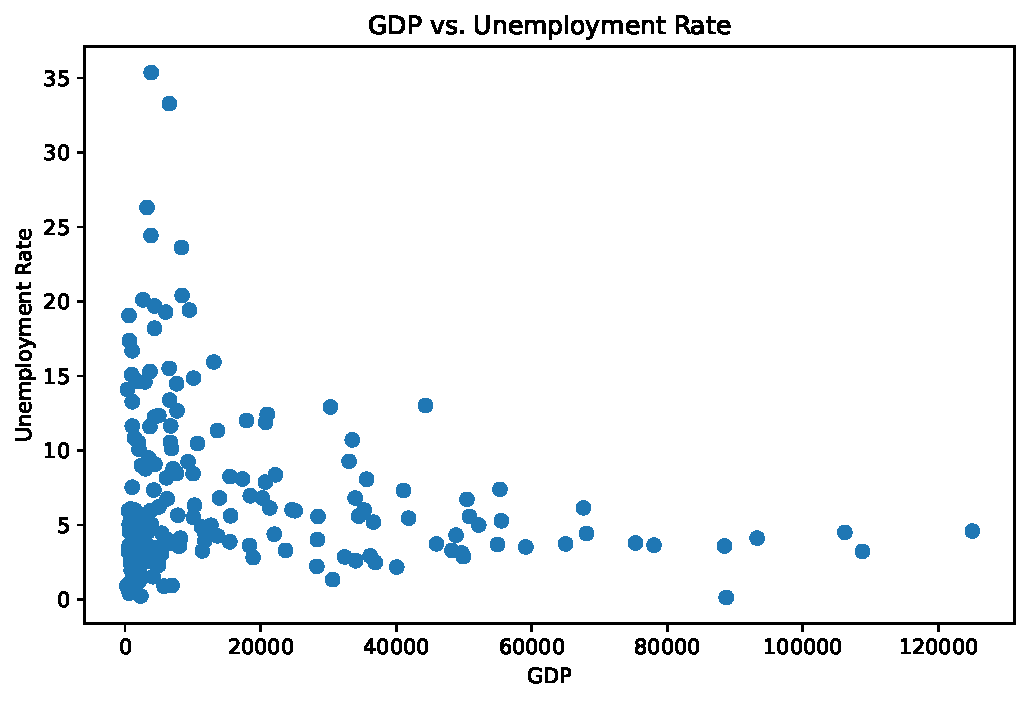
\includegraphics[keepaspectratio]{WDI_analysis_files/figure-pdf/cell-4-output-1.pdf}}

\begin{Shaded}
\begin{Highlighting}[]
\NormalTok{top\_countries }\OperatorTok{=}\NormalTok{ df\_wdi.sort\_values(by}\OperatorTok{=}\StringTok{"gdp\_per\_capita"}\NormalTok{, ascending}\OperatorTok{=}\VariableTok{False}\NormalTok{).head(}\DecValTok{10}\NormalTok{)}

\NormalTok{plt.figure(figsize}\OperatorTok{=}\NormalTok{(}\DecValTok{10}\NormalTok{,}\DecValTok{5}\NormalTok{))}
\NormalTok{plt.bar(top\_countries[}\StringTok{\textquotesingle{}country\textquotesingle{}}\NormalTok{], top\_countries[}\StringTok{\textquotesingle{}gdp\_per\_capita\textquotesingle{}}\NormalTok{], color}\OperatorTok{=}\StringTok{\textquotesingle{}royalblue\textquotesingle{}}\NormalTok{)}
\NormalTok{plt.title(}\StringTok{"Top 10 Countries by GDP"}\NormalTok{)}
\NormalTok{plt.xlabel(}\StringTok{"Country"}\NormalTok{)}
\NormalTok{plt.ylabel(}\StringTok{"GDP (in billion USD)"}\NormalTok{)}
\NormalTok{plt.xticks(rotation}\OperatorTok{=}\DecValTok{45}\NormalTok{)}
\NormalTok{plt.show()}
\end{Highlighting}
\end{Shaded}

\pandocbounded{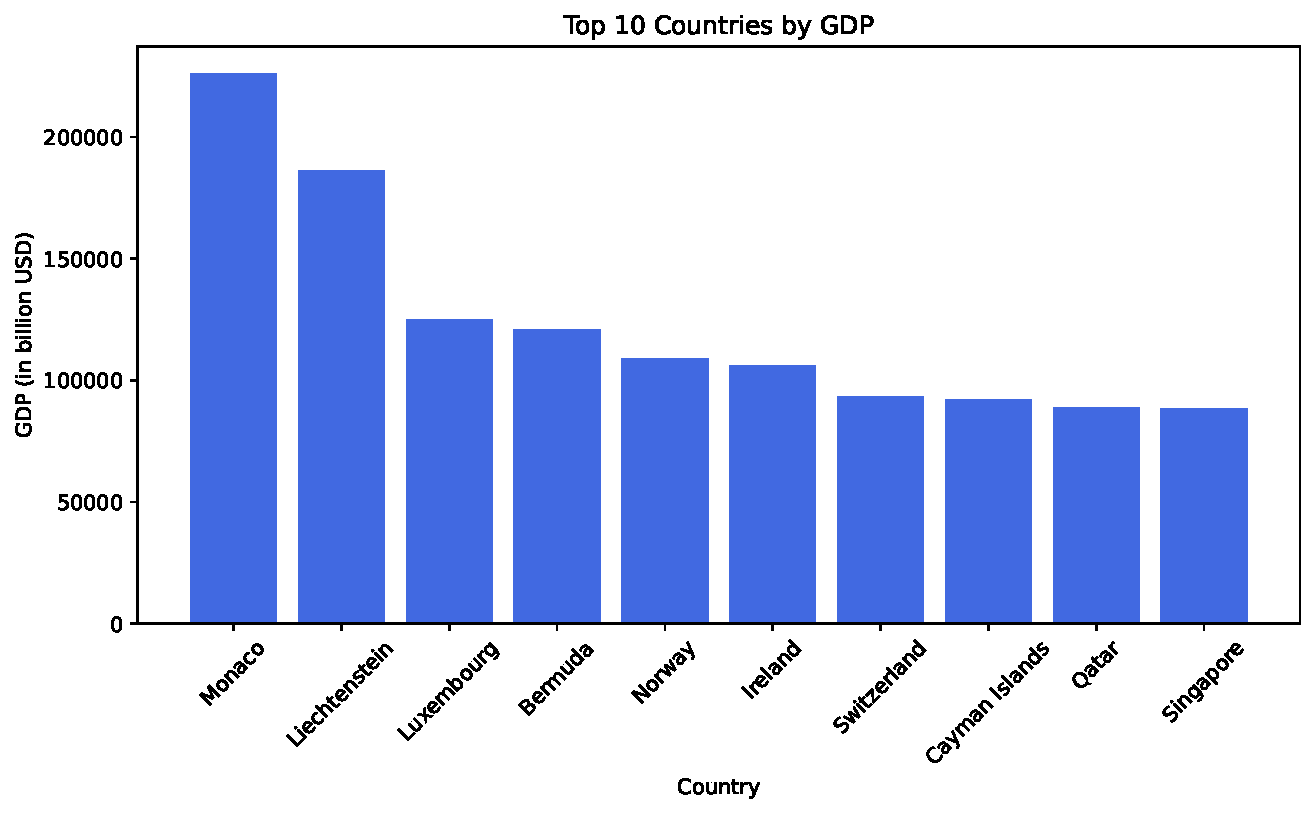
\includegraphics[keepaspectratio]{WDI_analysis_files/figure-pdf/cell-5-output-1.pdf}}

See Figure \textbf{?@fig-gdp-unemployment} for the GDP vs.~Unemployment
Rate scatter plot. Figure \textbf{?@fig-top-gdp} shows the GDP of the
top 10 countries.

\pandocbounded{\includegraphics[keepaspectratio]{gdp_vs_unemployment.png}}
\pandocbounded{\includegraphics[keepaspectratio]{top_gdp_chart.png}}

\begin{Shaded}
\begin{Highlighting}[]
\ImportTok{import}\NormalTok{ pandas }\ImportTok{as}\NormalTok{ pd}

\NormalTok{df\_wdi }\OperatorTok{=}\NormalTok{ pd.read\_csv(}\StringTok{"/Users/nicholasrichards/Desktop/QTM\_350/wdi.csv"}\NormalTok{)}

\NormalTok{table\_data }\OperatorTok{=}\NormalTok{ df\_wdi[[}\StringTok{\textquotesingle{}country\textquotesingle{}}\NormalTok{, }\StringTok{\textquotesingle{}gdp\_per\_capita\textquotesingle{}}\NormalTok{, }\StringTok{\textquotesingle{}life\_expectancy\textquotesingle{}}\NormalTok{, }
                     \StringTok{\textquotesingle{}education\_expenditure\_gdp\_share\textquotesingle{}}\NormalTok{, }\StringTok{\textquotesingle{}unemployment\_rate\textquotesingle{}}\NormalTok{]]}\OperatorTok{\textbackslash{}}
\NormalTok{                .sort\_values(by}\OperatorTok{=}\StringTok{\textquotesingle{}gdp\_per\_capita\textquotesingle{}}\NormalTok{, ascending}\OperatorTok{=}\VariableTok{False}\NormalTok{)}\OperatorTok{\textbackslash{}}
\NormalTok{                .head(}\DecValTok{10}\NormalTok{)}

\NormalTok{table\_data.style.set\_caption(}\StringTok{"Top 10 Countries by GDP per Capita"}\NormalTok{)}
\end{Highlighting}
\end{Shaded}

\begin{longtable}[]{@{}llllll@{}}
\caption{Top 10 Countries by GDP per
Capita}\label{T_5a4a1}\tabularnewline
\toprule\noalign{}
~ & country & gdp\_per\_capita & life\_expectancy &
education\_expenditure\_gdp\_share & unemployment\_rate \\
\midrule\noalign{}
\endfirsthead
\toprule\noalign{}
~ & country & gdp\_per\_capita & life\_expectancy &
education\_expenditure\_gdp\_share & unemployment\_rate \\
\midrule\noalign{}
\endhead
\bottomrule\noalign{}
\endlastfoot
130 & Monaco & 226052.001905 & nan & 1.173250 & nan \\
114 & Liechtenstein & 186400.233768 & 84.319512 & nan & nan \\
116 & Luxembourg & 125006.021815 & 83.046341 & 4.703022 & 4.588000 \\
21 & Bermuda & 120897.311155 & 81.571000 & 1.922213 & nan \\
147 & Norway & 108798.451166 & 82.560976 & 3.968020 & 3.231000 \\
93 & Ireland & 106194.755859 & 83.056098 & nan & 4.501000 \\
188 & Switzerland & 93245.795212 & 83.453659 & 4.888245 & 4.122000 \\
36 & Cayman Islands & 92202.147803 & nan & 1.488940 & nan \\
159 & Qatar & 88701.463350 & 81.559000 & nan & 0.130000 \\
171 & Singapore & 88428.702423 & 82.895122 & 2.488920 & 3.591000 \\
\end{longtable}

```

See Table \textbf{?@tbl-summary} for an overview. Figure
\textbf{?@fig-gdp-unemployment} shows the GDP-Unemployment relation.

Previous research indicates a complex relationship between life
expectancy and economic growth. Acemoglu and Johnson (2007) found that
increases in life expectancy have a nuanced impact on GDP growth
:contentReference{oaicite:2}. Similarly, Preston (2023) highlighted the
nonlinear effects of health improvements on economic performance
:contentReference{oaicite:3}.




\end{document}
